% ==============================================================================
% Modelo para Especificação de Requisitos de Software
% Prof. Vítor E. Silva Souza - NEMO/UFES :: DI/UFES :: PPGI/UFES
% Baseado em modelos cedidos pela Profª. Monalessa Perini Barcellos
%
% Baseado em abtex2-modelo-trabalho-academico.tex, v-1.9.2 laurocesar
% Copyright 2012-2014 by abnTeX2 group at http://abntex2.googlecode.com/ 
%
% This work may be distributed and/or modified under the conditions of the LaTeX 
% Project Public License, either version 1.3 of this license or (at your option) 
% any later version. The latest version of this license is in
% http://www.latex-project.org/lppl.txt.
%
% IMPORTANTE:
% Instruções encontram-se espalhadas pelo documento. Para facilitar sua leitura,
% tais instruções são precedidas por (*) -- utilize a função localizar do seu
% editor para passar por todas elas.
% ==============================================================================

% Usa o estilo abntex2, configurando detalhes de formatação e hifenização.
\documentclass[
12pt,				
oneside,		
a4paper,			
english,			% Idioma adicional para hifenização.
french,				% Idioma adicional para hifenização.
spanish,			% Idioma adicional para hifenização.
brazil				% O último idioma é o principal do documento.
]{abntex2}


%%% Importação de pacotes. %%%

% Conserta o erro "No room for a new \count". 
% O comando \reserveinserts deve ser comentado ou não, dependendo da versão do LaTeX.
\usepackage{etex}
%\reserveinserts{28}

% Usa a fonte Latin Modern.
\usepackage{lmodern}

% Seleção de códigos de fonte.
\usepackage[T1]{fontenc}

% Codificação do documento em Unicode.
\usepackage[utf8]{inputenc}

% Usado pela ficha catalográfica.
\usepackage{lastpage}

% Indenta o primeiro parágrafo de cada seção.
\usepackage{indentfirst}

% Controle das cores.
\usepackage[usenames,dvipsnames]{xcolor}

% Inclusão de gráficos.
\usepackage{graphicx}

% Melhor controle de leiaute de tabelas.
\usepackage{tabularx}
\usepackage{colortbl}
\usepackage{longtable}

% Adds PDF support to the environment landscape.
\usepackage{pdflscape}

% Inclusão de páginas em PDF diretamente no documento (para uso nos apêndices).
\usepackage{pdfpages}

% Para melhorias de justificação.
\usepackage{microtype}

% Citações padrão ABNT.
\usepackage[brazilian,hyperpageref]{backref}
\usepackage[alf]{abntex2cite}	
\renewcommand{\backrefpagesname}{Citado na(s) página(s):~}		% Usado sem a opção hyperpageref de backref.
\renewcommand{\backref}{}										% Texto padrão antes do número das páginas.
\renewcommand*{\backrefalt}[4]{									% Define os textos da citação.
	\ifcase #1
	Nenhuma citação no texto.
	\or
	Citado na página #2.
	\else
	Citado #1 vezes nas páginas #2.
	\fi}

% \rm is deprecated and should not be used in a LaTeX2e document
% http://tex.stackexchange.com/questions/151897/always-textrm-never-rm-a-counterexample
\renewcommand{\rm}{\textrm}

% Inclusão de símbolos não padrão.
\usepackage{amssymb}
\usepackage{eurosym}

% Para utilizar \eqref para referenciar equações.
\usepackage{amsmath}

% Permite mostrar figuras muito largas em modo paisagem com \begin{sidewaysfigure} ao invés de \begin{figure}.
\usepackage{rotating}

% Permite customizar listas enumeradas/com marcadores.
\usepackage{enumitem}

% Permite inserir hiperlinks com \url{}.
\usepackage{bigfoot}
\usepackage{hyperref}

% Permite usar o comando \hl{} para evidenciar texto com fundo amarelo. Útil para chamar atenção a itens a fazer.
\usepackage{soulutf8}

% Colorinlistoftodos package: to insert colored comments so authors can collaborate on the content.
% (*) Indicar o nome do aluno e substituir o nome do professor se for o caso.
\usepackage[colorinlistoftodos, textwidth=20mm, textsize=footnotesize]{todonotes}
\newcommand{\aluno}[1]{\todo[author=\textbf{Aluno},color=green!30,caption={},inline]{#1}}
\newcommand{\vitor}[1]{\todo[author=\textbf{Vítor},color=red!30,caption={},inline]{#1}}

% Permite inserir espaço em branco condicional (incluído no texto final só se necessário) em macros.
\usepackage{xspace}

% Permite inserir barreiras para que elementos flutuantes pendentes sejam colocados antes.
\usepackage{placeins}

% Permite incluir listagens de código com o comando \lstinputlisting{}.
\usepackage{listings}
\usepackage{caption}
\DeclareCaptionFont{white}{\color{white}}
\DeclareCaptionFormat{listing}{\colorbox{gray}{\parbox{\textwidth}{#1#2#3}}}
\captionsetup[lstlisting]{format=listing,labelfont=white,textfont=white}
\renewcommand{\lstlistingname}{Listagem}
\definecolor{mygray}{rgb}{0.5,0.5,0.5}
\lstset{
	basicstyle=\scriptsize,
	breaklines=true,
	numbers=left,
	numbersep=5pt,
	numberstyle=\tiny\color{mygray}, 
	rulecolor=\color{black},
	showstringspaces=false,
	tabsize=2,
	inputencoding=utf8,
	extendedchars=true,
	literate=%
	{é}{{\'{e}}}1
	{è}{{\`{e}}}1
	{ê}{{\^{e}}}1
	{ë}{{\¨{e}}}1
	{É}{{\'{E}}}1
	{Ê}{{\^{E}}}1
	{û}{{\^{u}}}1
	{ù}{{\`{u}}}1
	{â}{{\^{a}}}1
	{à}{{\`{a}}}1
	{á}{{\'{a}}}1
	{ã}{{\~{a}}}1
	{Á}{{\'{A}}}1
	{Â}{{\^{A}}}1
	{Ã}{{\~{A}}}1
	{ç}{{\c{c}}}1
	{Ç}{{\c{C}}}1
	{õ}{{\~{o}}}1
	{ó}{{\'{o}}}1
	{ô}{{\^{o}}}1
	{Õ}{{\~{O}}}1
	{Ó}{{\'{O}}}1
	{Ô}{{\^{O}}}1
	{î}{{\^{i}}}1
	{Î}{{\^{I}}}1
	{í}{{\'{i}}}1
	{Í}{{\~{Í}}}1
}




%%% Definição de variáveis. %%%
% (*) Substituir os textos abaixo com as informações apropriadas.
\titulo{Nome do Projeto}
\autor{Nome do Aluno}
\local{Vitória, ES}
\data{\the\year}

\instituicao{
	Universidade Federal do Espírito Santo -- UFES
	\par
	Centro Tecnológico
	\par
	Departamento de Informática}
\newcommand{\subtitulo}{Documento de Requisitos de Sistema}
\newcommand{\versao}{1.0}

% Define a capa.
\renewcommand{\imprimircapa}{%
	\begin{capa}%
		\center
		
		{\ABNTEXchapterfont\large\subtitulo{}}
		\vfill
		\begin{center}
			\ABNTEXchapterfont\bfseries\LARGE\imprimirtitulo
		\end{center}
		
		\vfill
		\large\imprimirlocal
		\linebreak
		\large\imprimirdata
		\vspace*{1cm}
	\end{capa}
}

% Macros específicas do trabalho.
% (*) Inclua aqui termos que são utilizados muitas vezes e que demandam formatação especial.
% Exemplo: Java com TM (trademark) em superscript.
% Use sempre \xspace para que o LaTeX inclua espaço em branco após a macro somente quando necessário.
\newcommand{\java}{Java\texttrademark\xspace}




%%% Configurações finais de aparência. %%%

% Altera o aspecto de algumas cores.
\definecolor{blue}{RGB}{41,5,195}
\definecolor{lightgray}{gray}{0.9}

% Informações do PDF.
\makeatletter
\hypersetup{
	pdftitle={\@title}, 
	pdfauthor={\@author},
	pdfsubject={\imprimirpreambulo},
	pdfcreator={LaTeX with abnTeX2},
	pdfkeywords={abnt}{latex}{abntex}{abntex2}{trabalho acadêmico}, 
	colorlinks=true,				% Colore os links (ao invés de usar caixas).
	linkcolor=blue,					% Cor dos links.
	citecolor=blue,					% Cor dos links na bibliografia.
	filecolor=magenta,				% Cor dos links de arquivo.
	urlcolor=blue,					% Cor das URLs.
	bookmarksdepth=4
}
\makeatother

% Espaçamentos entre linhas e parágrafos.
\setlength{\parindent}{1.3cm}
\setlength{\parskip}{0.2cm}



%%% Páginas iniciais do documento: capa, folha de rosto, ficha, resumo, tabelas, etc. %%%

% Compila o índice.
\makeindex

% Inicia o documento.
\begin{document}

% Retira espaço extra obsoleto entre as frases.
\frenchspacing

% Inclui o brasão da UFES.
\begin{figure}[h]
	\centering
	
\includegraphics[scale=0.055]{brasao.jpg}
	\label{ppts3}
\end{figure} 

% Capa do trabalho.
\imprimircapa

% (*) Incluir linhas no registro de alterações a cada nova versão.
\begin{center}
	{\large\bfseries Registro de Alterações:}
	
	\vspace{0.5cm}
	\begin{tabular}{|c|p{45mm}|c|p{60mm}|} \hline
		
		\textbf{Versão} & \textbf{Responsável} & \textbf{Data}  & \textbf{Alterações} \\ \hline   
		
		1.0  & Nome do Responsável & dd/MM/yyyy & Versão inicial. \\\hline 
	\end{tabular}
\end{center}
\newpage



%%% Início da parte de conteúdo do documento. %%%
% Marca o início dos elementos textuais.
\textual

% Inclusão dos capítulos como seções (sem quebra de página).
\begingroup
\let\clearpage\relax

% ==============================================================================
% TCC - Nome do Aluno
% Capítulo 1 - Introdução
% ==============================================================================
\chapter{Introdução}
\label{sec-intro}

\hl{Texto.}

\hrulefill

Além do template pronto para uso, este documento inclui exemplos de uso de \latex que podem ser úteis para aqueles que possuem pouca experiência com a ferramenta. Quando for começar a escrever seu PG, apague todo o conteúdo abaixo da palavra ``Texto''.



%%% Início de seção. %%%
\section{Seções e subseções}
\label{sec-intro-secoes}

O documento é organizado em capítulos (\texttt{\textbackslash chapter\{\}}), seções (\texttt{\textbackslash section\{\}}), subseções (\texttt{\textbackslash subsection\{\}}), sub-subseções (\texttt{\textbackslash subsubsection\{\}}) e assim por diante. Atenção, porém, a não criar estruturas muito profundas (sub-sub-sub-...) pois o documento não fica bem estruturado.


%%% Início de seção. %%%
\subsection{Referências a seções}
\label{sec-intro-secoes-refs}

Cada parte do documento (capítulo, seção, etc.) deve possuir um rótulo logo abaixo de sua definição. Por exemplo, este capítulo é definido com \texttt{\textbackslash chapter\{Introdução\}} seguido por \texttt{\textbackslash label\{sec-intro\}}. Assim, podemos fazer referências cruzadas usando o comando \texttt{\textbackslash ref\{rótulo\}}: ``O Capítulo~\ref{sec-intro} começa com a Seção~\ref{sec-intro-secoes}, que é ainda subdividida nas subseções~\ref{sec-intro-secoes-refs} e~\ref{sec-intro-secoes-sobrerefs}.

Para melhor organização das partes do documento, sugere-se primeiro utilizar o prefixo \texttt{sec-} (para diferenciar de referências à figuras, tabelas, etc. quando usarmos o comando \texttt{\textbackslash ref\{\}}) e também representar a hierarquia das seções nos rótulos. Por exemplo, o Capítulo~\ref{sec-intro} tem rótulo \texttt{sec-intro}, sua Seção~\ref{sec-intro-secoes} tem rótulo \texttt{sec-intro-secoes} e a Subseção~\ref{sec-intro-secoes-refs} tem rótulo \texttt{sec-intro-secoes-refs}.



%%% Início de seção. %%%
\subsection{Sobre referências cruzadas}
\label{sec-intro-secoes-sobrerefs}

Nas próximas seções, veremos que é possível fazer referência cruzada não só a seções mas também a listagens de código, figuras, tabelas, etc. Em todos estes casos, quando nos referimos à Seção X, Listagem Y ou Figura Z, consideramos que estes são os nomes próprios destes elementos e, portanto, usa-se a primeira letra maiúscula. Isso pode ser visto na Subseção~\ref{sec-intro-secoes-refs}, acima. A exceção é quando nos referimos a vários elementos ao mesmo tempo, por exemplo: ``as subseções~\ref{sec-intro-secoes-refs} e~\ref{sec-intro-secoes-sobrerefs}''.

Por fim, ao usar o comando \texttt{\textbackslash ref\{\}}, sugere-se separá-lo da palavra que vem antes dele com um \textasciitilde\ ao invés de espaço. Por exemplo: \texttt{o capítulo\textasciitilde \textbackslash ref\{sec-intro\}}. Isso faz com que o \latex não quebre linha entre a palavra \texttt{capítulo} e o número do capítulo.




%%% Início de seção. %%%
\section{Citações bibliográficas}
\label{sec-intro-citacoes}

Este documento utiliza a ferramenta de gerenciamento de referências bibliográficas do \latex, chamada \emph{BibTeX}. O arquivo \texttt{bibliografia.bib}, referenciado no arquivo \latex principal deste documento, contém algumas referências bibliográficas de exemplo. Assim como capítulos, seções, etc., tais referências também possuem rótulos, especificados como primeiro parâmetro de cada entrada (ex.: \texttt{@incollection\{souza-et-al:iism08, ...\}}.

Sugere-se um padrão para rótulos de referências bibliográficas para que fique claro também no código \latex qual referência está sendo citada. Por exemplo, ao citar a referência \texttt{souza-et-al:sesas13}, sabemos que é um artigo escrito por \emph{Souza} e outros, publicado no \emph{SESAS} em \emph{2013} (geralmente a pessoa que citou sabe que publicação é SESAS e quem é Souza).

Para citar uma referência bibliográfica contida no arquivo \emph{BibTeX}, basta usar seu rótulo como parâmetro de um de dois comandos possíveis de citação:

\begin{itemize}
	\item O comando \texttt{\textbackslash cite\{\}} efetua uma citação tradicional, colocando o nome do(s) autor(es) e o ano entre parênteses. Por exemplo, \texttt{\textbackslash cite\{souza-et-al:iism08\}} é transformado em \cite{souza-et-al:iism08};
	
	\item O comando \texttt{\textbackslash citeonline\{\}} efetua uma citação integrada ao texto, colocando o nome do(s) autor(es) direto no texto e somente o ano entre parênteses. Por exemplo, ``de acordo com \texttt{\textbackslash citeonline\{souza-et-al:iism08\}}'' é transformado em: de acordo com \citeonline{souza-et-al:iism08};
\end{itemize}

Também é possível citar vários trabalhos de uma só vez, separando os rótulos das referências bibliográficas com uma vírgula dentro do comando apropriado. Por exemplo, \texttt{\textbackslash cite\{souza-et-al:sesas13,souza-et-al:csrd13\}} \cite{souza-et-al:sesas13,souza-et-al:csrd13}.

Os trabalhos citados são automaticamente incluídos na seção de referências bibliográficas, ao final do documento. Tudo é formatado automaticamente segundo padrões da ABNT.



%%% Início de seção. %%%
\section{Listagens de código}
\label{sec-intro-listagens}

O pacote \texttt{listings}, incluído neste template, permite a inclusão de listagens de código. Análogo ao já feito anteriormente, listagens possuem rótulos para que possam ser referenciadas e sugerimos uma regra de nomenclatura para tais rótulos: usar como prefixo o rótulo do capítulo, substituindo \texttt{sec-} por \texttt{lst-}.

A Listagem~\ref{lst-intro-exemplo}, por exemplo, possui o rótulo \texttt{lst-intro-exemplo} e representa o código que foi usado no próprio documento para exibir as listagens desta seção. Como podemos ver, a sugestão é que os arquivos de código sejam colocados dentro da pasta \texttt{codigos/} e tenham nome idêntico ao rótulo, colocando a extensão adequada ao tipo de código.

\lstinputlisting[label=lst-intro-exemplo, caption=Exemplo de código \latex para inclusão de listagens de código., float=htpb]{codigos/lst-intro-exemplo.tex}

A Listagem~\ref{lst-intro-outroexemplo} mostra um exemplo de listagem com especificação da linguagem utilizada no código. O pacote \texttt{listings} reconhece algumas linguagens\footnote{Veja a lista de linguagens suportadas em \url{http://en.wikibooks.org/wiki/LaTeX/Source\_Code\_Listings\#Supported_languages}.} e faz ``coloração'' de código (na verdade, usa \textbf{negrito} e não cores) de acordo com a linguagem. O parâmetro \texttt{float=htpb} incluído em ambos os exemplos impede que a listagem seja quebrada em diferentes páginas.

\lstinputlisting[label=lst-intro-outroexemplo, caption=Exemplo de código \java especificando linguagem utilizada., language=Java, float=htpb]{codigos/lst-intro-outroexemplo.java}



%%% Início de seção. %%%
\section{Figuras}
\label{sec-intro-figuras}

Figuras podem ser inseridas no documento usando o \emph{ambiente} \texttt{figure} (ou seja, \texttt{\textbackslash begin\{figure\}} e \texttt{\textbackslash end\{figure\}}) e o comando \texttt{\textbackslash includegraphics\{\}}. Existem alguns outros elementos e propriedades úteis de serem configuradas, resultando no código exibido na Listagem~\ref{lst-intro-figuras}.

\lstinputlisting[label=lst-intro-figuras, caption=Código \latex utilizado para inclusão das figuras na Seção~\ref{sec-intro-figuras}., float=htpb]{codigos/lst-intro-figuras.tex}

O comando \texttt{\textbackslash centering} centraliza a figura na página. A opção \texttt{width} do comando \texttt{\textbackslash includegraphics\{\}} determina o tamanho da figura e usa-se \texttt{\textbackslash textwidth} (opcionalmente multiplicado por um número) para se referir à largura da página.

O parâmetro do comando \texttt{\textbackslash includegraphics\{\}} indica onde a imagem pode ser encontrada. Foi criado o diretório \texttt{figuras/} para conter as figuras do documento, dando uma melhor organização aos arquivos. Ao abrir esta pasta, repare que as figuras possuem duas versões---uma em \texttt{.eps} e outra em \texttt{.pdf}---e que o comando \texttt{\textbackslash includegraphics\{\}} não especifica a extensão. Isso se dá porque o \latex possui um compilador para formato PostScript (\texttt{latex}) que espera as imagens em \texttt{.eps} e um compilador para PDF (\texttt{pdflatex}) que espera as imagens em \texttt{.pdf}. Dependendo do seu ambiente \latex, é possível apenas colocar as figuras em formatos mais comuns, como JPG ou PNG e ele incluir no PDF sem problemas. Vale a pena testar.

Por fim, o comando \texttt{\textbackslash caption\{\}} especifica a descrição da figura e \texttt{\textbackslash label\{\}}, como de costume, estabelece um rótulo para permitir referência cruzada de figuras. Note ainda que é utilizada a mesma estratégia de nomenclatura de rótulos usada nas listagens, porém utilizando o prefixo \texttt{fig-}.

As figuras~\ref{fig-intro-nemologo} e~\ref{fig-intro-exemplosideways} mostram o resultado do código da Listagem~\ref{lst-intro-figuras}. A Figura~\ref{fig-intro-exemplosideways}, em particular, utiliza o pacote \texttt{rotating} para mostrar figuras largas em modo paisagem. Basta usar o ambiente \texttt{sidewaysfigure} ao invés de \texttt{figure}.

\begin{figure}
	\centering
	
\includegraphics[width=.25\textwidth]{figuras/fig-intro-nemologo} 
	\caption{Exemplo de figura: logo do Nemo.}
	\label{fig-intro-nemologo}
\end{figure}

\begin{sidewaysfigure}
	\centering
	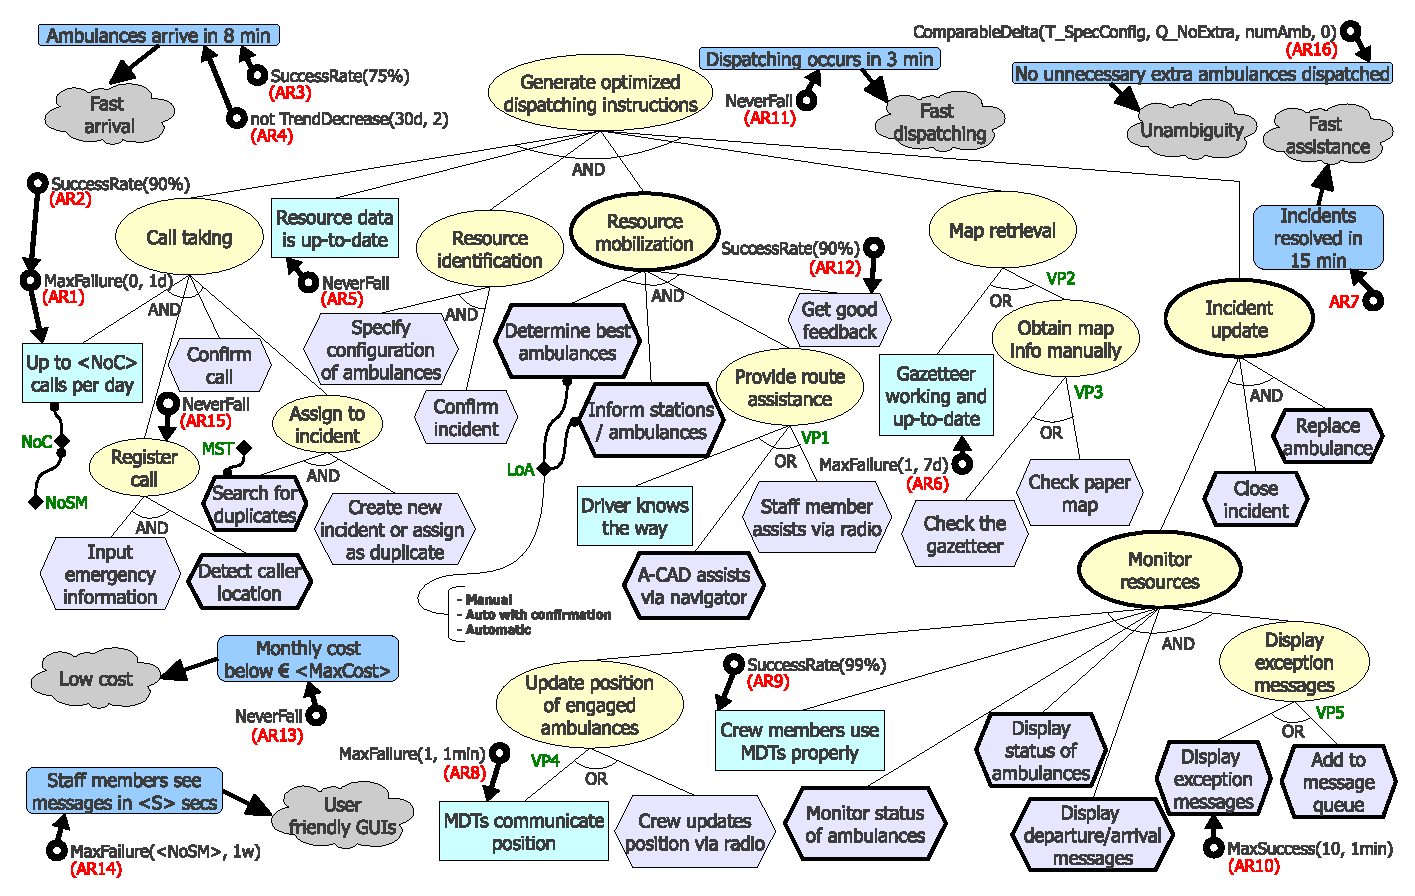
\includegraphics[width=\textwidth]{figuras/fig-intro-exemplosideways} 
	\caption{Exemplo de figura em modo paisagem: um modelo de objetivos~\cite{souza-mylopoulos:spe13}.}
	\label{fig-intro-exemplosideways}
\end{sidewaysfigure}



%%% Início de seção. %%%
\section{Tabelas}
\label{sec-intro-tabelas}

Tabelas são um ponto fraco do \latex. Elas são complicadas de fazer e, dependendo da complexidade da tabela (muitas células mescladas, por exemplo), vale a pena construi-las em outro programa (por exemplo, em seu editor de texto favorito) e inclui-las no documento como figuras. Mostramos, no entanto, alguns exemplos de tabela a seguir. O código utilizado para criar as tabelas encontra-se nas listagens~\ref{lst-intro-tabelas01}, \ref{lst-intro-tabelas02} e~\ref{lst-intro-tabelas03}.

\lstinputlisting[label=lst-intro-tabelas01, caption=Código \latex utilizado para inclusão das tabelas~\ref{tbl-intro-exemplo01} e~\ref{tbl-intro-exemplo02}., float=htpb]{codigos/lst-intro-tabelas01.tex}

\lstinputlisting[label=lst-intro-tabelas02, caption=Código \latex utilizado para inclusão da Tabela~\ref{tbl-intro-exemplo03}., float=htpb]{codigos/lst-intro-tabelas02.tex}

\lstinputlisting[label=lst-intro-tabelas03, caption=Código \latex utilizado para inclusão da Tabela~\ref{tbl-intro-exemplo04}., float=htpb]{codigos/lst-intro-tabelas03.tex}

Em particular, a Tabela~\ref{tbl-intro-exemplo04} utiliza um pacote chamado \texttt{tabularx}, que permite maior controle do layout das tabelas. Ao definir o ambiente \texttt{\textbackslash begin\{tabularx\}}, são definidos os tamanhos de cada coluna proporcional à largura ocupada pela tabela. Veja na Listagem~\ref{lst-intro-tabelas03} que as primeiras duas colunas não definem o atributo \texttt{\textbackslash hsize}, o que faz com que elas fiquem com o tamanho padrão de coluna, que é a largura da tabela dividida pelo número de colunas. Já a terceira coluna define \texttt{\textbackslash hsize=1.2\textbackslash hsize}, ou seja, esta coluna deve ser 20\% maior do que o tamanho padrão. Para isso, é preciso retirar de outras colunas, portanto a quarta e quinta colunas são definidas como 10\% menores (ou seja, \texttt{\textbackslash hsize=0.9\textbackslash hsize}).

% Exemplo de tabela 01:
\begin{table}
	\caption{Exemplo de tabela com diferentes alinhamentos de conteúdo.}
	\label{tbl-intro-exemplo01}
	\centering
	\begin{tabular}{ | c | l | r | p{40mm} |}\hline
		\textbf{Centralizado} & \textbf{Esquerda} & \textbf{Direita} & \textbf{Parágrafo}\\\hline
		C & L & R & Alinhamento de tipo parágrafo especifica largura da coluna e quebra o texto automaticamente.\\
		\hline
		Linha 2 & Linha 2 & Linha 2 & Linha 2\\
		\hline
	\end{tabular}
\end{table}

% Exemplo de tabela 02:
\begin{table}
	\caption{Exemplo que especifica largura de coluna e usa lista enumerada (adaptada de~\cite{souza-mylopoulos:spe13}).}
	\label{tbl-intro-exemplo02}
	\centering
	\renewcommand{\arraystretch}{1.2}
	\begin{small}
		\begin{tabular}{ | p{15mm} | p{77mm} | p{55mm} |}\hline
			\textbf{\textit{AwReq}} & \textbf{Adaptation strategies} & \textbf{Applicability conditions}\\\hline
			
			AR1 &
			\vspace{-2mm}\begin{enumerate}[topsep=0cm, partopsep=0cm, itemsep=0cm, parsep=0cm, leftmargin=0.5cm]
				\item \textit{Warning(``AS Management'')}
				\item \textit{Reconfigure($\varnothing$)}
			\end{enumerate}\vspace{-4mm} &
			\vspace{-2mm}\begin{enumerate}[topsep=0cm, partopsep=0cm, itemsep=0cm, parsep=0cm, leftmargin=0.5cm]
				\item Once per adaptation session;
				\item Always.
			\end{enumerate}\vspace{-4mm}
			\\\hline
			
			AR2 &
			\vspace{-2mm}\begin{enumerate}[topsep=0cm, partopsep=0cm, itemsep=0cm, parsep=0cm, leftmargin=0.5cm]
				\item \textit{Warning(``AS Management'')}
				\item \textit{Reconfigure($\varnothing$)}
			\end{enumerate}\vspace{-4mm} &
			\vspace{-2mm}\begin{enumerate}[topsep=0cm, partopsep=0cm, itemsep=0cm, parsep=0cm, leftmargin=0.5cm]
				\item Once per adaptation session;
				\item Always.
			\end{enumerate}\vspace{-4mm}
			\\\hline
		\end{tabular}
	\end{small}
\end{table}

% Exemplo de tabela 03:
\begin{table}
	\caption{Exemplo que mostra equações em duas colunas (adaptada de~\cite{souza-mylopoulos:spe13}).}
	\label{tbl-intro-exemplo03}
	\centering
	\vspace{1mm}
	\fbox{\begin{minipage}{.98\linewidth}
			\begin{minipage}{0.51\linewidth}
				\vspace{-4mm}
				\begin{eqnarray}
				\Delta \left( I_{AR1} / NoSM \right) \left[ 0, maxSM \right] > 0\\
				\Delta \left( I_{AR2} / NoSM \right) \left[ 0, maxSM \right] > 0\\
				\Delta \left( I_{AR3} / LoA \right) < 0\\
				\end{eqnarray}
				\vspace{-6mm}
			\end{minipage}
			\hspace{2mm}
			\vline 
			\begin{minipage}{0.41\linewidth}
				\vspace{-4mm}
				\begin{eqnarray}
				\Delta \left( I_{AR11} / VP2 \right) < 0\\
				\Delta \left( I_{AR12} / VP2 \right) > 0\\
				\Delta \left( I_{AR6} / VP3 \right) > 0\\
				\end{eqnarray}
				\vspace{-6mm}
			\end{minipage}
	\end{minipage}}
\end{table}

% Exemplo de tabela 04:
\begin{table}[h]
	\caption{Exemplo que utiliza o pacote \texttt{tabularx}, extraído de um artigo ainda não publicado.}
	\label{tbl-intro-exemplo04}
	\centering\tiny\def\tabularxcolumn#1{m{#1}}
	\begin{tabularx}{\columnwidth}{ >{\centering}X | >{\centering}X | >{\hsize=1.2\hsize\centering}X | >{\hsize=0.9\hsize\centering}X | >{\hsize=0.9\hsize\centering\arraybackslash}X }
		\hline
		\textbf{Applied Criteria} & \textbf{Analyzed Content} & \textbf{Initial\\Occurrences} & \textbf{Final Results} & \textbf{Reduction (\%)} \\
		\hline
		Duplicate Removal & Title, authors and year & 903 & 420 & 54,84\% \\ 
		\hline 
		IC and ECs & Title, abstract and keywords & 420 & 130 & 69,05\% \\ 
		\hline 
		IC and ECs & Full text & 130 & 117 & 10\% \\ 
		\hline 
		Final Results & -- & 903 & 117 & 87,04\% \\ 
		\hline 
	\end{tabularx}
\end{table}
\vspace*{1.5cm}

\chapter{Definição de Requisitos}
\label{sec-requisitos}
\vspace{-1cm}

Esta seção descreve o resultado da atividade de levantamento de requisitos.
A Subseção~\ref{sec-requisitos-minimundo} descreve o minimundo do sistema e seu propósito, apresentando superficialmente suas principais características. 
A Subseção~\ref{sec-requisitos-usuario} lista os requisitos de usuário do sistema, na forma de estórias de usuário e requisitos não-funcionais. 




\section{Descrição do Minimundo e do Propósito do Sistema}
\label{sec-requisitos-minimundo}

\vitor{De forma detalhada (vários parágrafos, possivelmente dividir em subseções), descrever o minimundo do sistema, ou seja, o domínio no qual ele se encaixa e quais os problemas que pretende resolver. Descrever também por meio de quais funcionalidades o sistema resolverá os problemas, justificando, assim, sua existência.}



\section{Requisitos de Usuário}
\label{sec-requisitos-usuario}

\vitor{Listar os principais \textit{stakeholders} do projeto no parágrafo abaixo e preencher as tabelas de estórias de usuário, requisitos não-funcionais e regras de negócio, com atenção aos identificadores e \textit{labels}. Ao preencher as lacunas, remover a marcação em amarelo (comando \textbackslash hl\{\} no \LaTeX).}

Tomando por base o contexto do sistema descrito na Seção~\ref{sec-requisitos-minimundo} e considerando como principais \textit{stakeholders} \hl{(listar aqui os principais stakeholders do projeto)}, foram identificadas estórias de usuário e requisitos não-funcionais.

As estórias de usuário são apresentadas na Tabela~\ref{tbl-requisitos-uss} e os requisitos não-funcionais globais (ou seja, aqueles que não são caracterizados como critérios de aceitação de estórias de usuário específicas) na Tabela~\ref{tbl-requisitos-rnfs}.

% Define contador e identificador para estórias de usuário.
\newcounter{uscount}
\renewcommand*\theuscount{US-\arabic{uscount}}
\newcommand*\US{\refstepcounter{uscount}\theuscount}
\setcounter{uscount}{0}

% Define uma macro para as linhas de user stories.
% Usar \userstory{label}{dependências}{prioridade}{descrição}{critérios de qualidade (usando \item)}.
\newcommand{\userstory}[5]{
	\\\hline
	\cellcolor{lightgray}\textbf{ID:} & \US\label{#1} & 
	\cellcolor{lightgray}\textbf{Depende:} & #2 & 
	\cellcolor{lightgray}\textbf{Prioridade:} & #3 \\\hline
	\cellcolor{lightgray}\textbf{Descrição:} & 
	\multicolumn{5}{|p{12cm}|}{#4}\\\hline
	\cellcolor{lightgray}\parbox{2.5cm}{\raggedleft \textbf{Critérios de\\Aceitação:}} & 
	\multicolumn{5}{|p{12cm}|}{
		\parbox{12cm}{
			\begin{enumerate}[leftmargin=15mm,label=-- CA\arabic*:]\itemsep-2mm
				#5
			\end{enumerate}
		}		
	}\\\hline
	\multicolumn{6}{c}{}
}

\vitor{A Tabela~\ref{tbl-requisitos-uss} traz exemplos de estórias de usuário: genérico (\ref{us-exemplo-generico}), de cadastro/CRUD (\ref{us-exemplo-cadastro}) e de consulta (\ref{us-exemplo-consulta}). Note que:
	\begin{itemize}
		\item As estórias possuem um \textit{label} (ex.: \texttt{us-exemplo-generico}). Sugere-se não utilizar números sequenciais (ex.: \texttt{us-01}, \texttt{us-02}, etc.) mas sim algo que identifique aquela estória (ex.: \texttt{us-cadastrar-usuarios}); 
		\item Há um padrão de critérios de aceitação para estórias de cadastro e de consulta. Sugere-se seguir o padrão, preenchendo as lacunas e ajustando onde necessário;
		\item As dependências são especificadas por meio dos IDs das outras estórias de usuário das quais aquela estória depende, separadas por vírgula;
		\item Já a prioridade deve ser especificada com um dos seguintes valores: Alta, Média ou Baixa.
	\end{itemize}}

\begin{longtable}{|r|p{1.3cm}|r|p{4cm}|r|p{1.3cm}|}
\caption{Estórias de Usuário.}
\label{tbl-requisitos-uss}

% Especificar as estórias de usuário abaixo, utilizando a macro, substituindo os exemplos.
\userstory{us-exemplo-generico}{}{Baixa}
{Como \hl{ator}, quero \hl{função}, para \hl{finalidade}. \hl{(Genérico)}}
{
\item Critério de aceitação 1;
\item Critério de aceitação 2;
\item Critério de aceitação N.
}

\userstory{us-exemplo-cadastro}{\ref{us-exemplo-generico}}{Média}
{Como \hl{ator}, quero cadastrar \hl{objeto}, para \hl{finalidade}.  \hl{(Cadastro)}}
{
\item O sistema deve prover funcionalidades ``CRUD'';
\item No cadastro (C), devem ser informados: \hl{campos obrigatórios}. Opcionalmente, podem ser informados: \hl{campos opcionais}. O sistema deve registrar automaticamente: \hl{campos com valores gerados automaticamente, se houver};
\item Na listagem (R), devem ser exibidos: \hl{campos}. Pode-se ordernar por: \hl{campos, se houver}. Pode-se filtrar por: \hl{campos, se houver};
\item Na visualização (R), devem ser exibidos todos os dados elencados no cadastro, além de: \hl{campos extras, se houver};
\item Na atualização (U), podem ser modificados todos os dados, exceto: \hl{campos imutáveis}. Deve-se respeitar aqueles indicados como obrigatórios no cadastro (não podem ser alterados para valores vazios). O sistema deve registrar automaticamente: \hl{campos com valores atualizados automaticamente, se houver};
\item Na exclusão (D), devem ser excluídos também: \hl{objetos subordinados ao objeto que está sendo excluído, que serão excluídos em cascata};
\item A exclusão (D) não deve ser permitida quando: \hl{descrição das situações, geralmente quando o objeto está associado a outros que não serão excluídos em cascata};
\item Os dados devem ser validados no cadastro e na atualização e o sistema deve exibir mensagens de erro informativas no caso de dados inválidos.
}

\userstory{us-exemplo-consulta}{\ref{us-exemplo-generico}, \ref{us-exemplo-cadastro}}{Alta}
{Como \hl{ator}, quero consultar \hl{informações}, para \hl{finalidade}. \hl{(Consulta)}}
{
\item Para realizar a consulta, o usuário deve informar como parâmetros: \hl{parâmetros};
\item Devem ser apresentadas as seguintes informações para o usuário: \hl{objetos e seus dados, relacionados aos parâmetros informados}.
}
\end{longtable}

\vitor{A Tabela~\ref{tbl-requisitos-rnfs} deve ser preenchida com os requisitos não-funcionais, seguindo as mesmas recomendações quanto aos \textit{labels} e quanto à prioridade feita para as estórias de usuário. Na coluna \textbf{Categoria}, sugere-se usar características de qualidade definidas pelo modelo de qualidade de produtos de software da norma ISO/IEC 25010, conforme discutido por Falbo em suas Notas de Aula de Projeto de Sistemas, Seção 2.3.}

% Define contador e identificador para requisitos não funcionais.
% Usar \RNF\label{rnf-nome-do-label} para cada requisito definido.
\newcounter{rnfcount}
\renewcommand*\thernfcount{RNF-\arabic{rnfcount}}
\newcommand*\RNF{\refstepcounter{rnfcount}\thernfcount}
\setcounter{rnfcount}{0}

% Tabela de requisitos não funcionais.
\begin{longtable}{|c|p{8.3cm}|c|c|}
	\caption{Requisitos Não Funcionais.}
	\label{tbl-requisitos-rnfs} \\\hline 
	
	% Cabeçalho e repetição do mesmo em cada nova página. Manter como está.
	\rowcolor{lightgray}
	\textbf{ID} & \textbf{Descrição} & \textbf{Categoria} & \textbf{Prioridade} \\\hline		
	\endfirsthead
	\hline
	\rowcolor{lightgray}
	\textbf{ID} & \textbf{Descrição} & \textbf{Categoria} & \textbf{Prioridade} \\\hline		
	\endhead
	
	% Especificar os requisitos abaixo, substituindo os exemplos.
	\RNF\label{rnf-exemplo-primeiro} & Descrição sucinta. & Característica & Baixa \\\hline 	

	\RNF\label{rnf-exemplo-segundo} & Descrição sucinta. & de & Média \\\hline 	

	\RNF\label{rnf-exemplo-terceiro} & Descrição sucinta. & qualidade & ou Alta \\\hline
\end{longtable}

\FloatBarrier

\vspace*{1.5cm}

\chapter{Identificação de Subsistemas}
\label{sec-subsistemas}
\vspace{-1cm}

\vitor{Listar a quantidade e o nome dos subsistemas no parágrafo abaixo, substituir a Figura~\ref{fig-subsistemas} pelo diagrama de pacotes do sistema, ilustrando os subsistemas e suas interdependências, e preencher a Tabela~\ref{tbl-subsistemas} com as descrições dos subsistemas.}

Para atender aos requisitos elencados na Seção~\ref{sec-requisitos} e a fim de facilitar o gerenciamento do projeto, o sistema foi dividido em \hl{3} subsistemas: \hl{Subsistema 01, Subsistema 02 e Subsistema 03}. 

A Figura~\ref{fig-subsistemas} ilustra os subsistemas e suas interdependências, enquanto a Tabela~\ref{tbl-subsistemas} apresenta uma breve descrição de cada subsistema identificado.

\begin{figure}
	\centering
	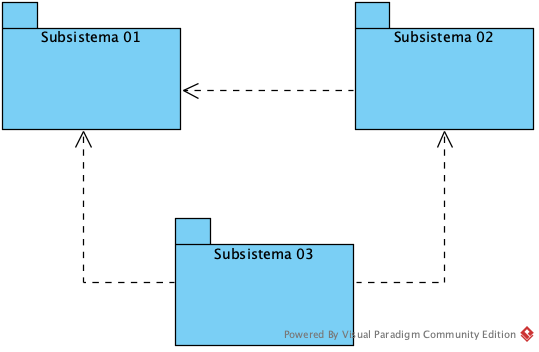
\includegraphics[width=.5\textwidth]{figuras/fig-subsistemas.png}
	\caption{Diagrama de Pacotes e os Subsistemas Identificados.}
	\label{fig-subsistemas}
\end{figure} 


% Tabela de subsistemas.
\begin{longtable}{|p{3cm}|p{12cm}|}
	\caption{Subsistemas identificados e suas interdependências.}
	\label{tbl-subsistemas} \\\hline 
	
	% Cabeçalho e repetição do mesmo em cada nova página. Manter como está.
	\rowcolor{lightgray}
	\textbf{Subsistema} & \textbf{Descrição} \\\hline		
	\endfirsthead
	\hline
	\rowcolor{lightgray}
	\textbf{Subsistema} & \textbf{Descrição} \\\hline		
	\endhead
	
	% Especificar os subsistemas abaixo, substituindo os exemplos.
	Subsistema 01 & Descrição do subsistema 01. \\\hline
	
	Subsistema 02 & Descrição do subsistema 02. \\\hline
	
	Subsistema 03 & Descrição do subsistema 03. \\\hline
\end{longtable}


\vspace*{1.5cm}

\chapter{Modelo de Casos de Uso}
\label{sec-casos-de-uso}

% Define contador e identificador para casos de uso.
% Usar \UC\label{rf-nome-do-label} para cada caso de uso definido.
\newcounter{uccount}
\renewcommand*\theuccount{UC-\arabic{uccount}}
\newcommand*\UC{\refstepcounter{uccount}\theuccount}
\setcounter{uccount}{0}

\vitor{Listar e descrever os atores na Tabela~\ref{tbl-casos-de-uso-atores}. Criar uma subseção para cada subsistema e, dentro dela, apresentar o diagrama de casos de uso (ex.: Figura~\ref{fig-casos-de-uso-subsistema-01}), a tabela de casos de uso cadastrais (ex.: Tabela~\ref{tbl-casos-de-uso-subsistema-01-cruds}), a tabela de casos de uso de consulta (ex.: Tabela~\ref{tbl-casos-de-uso-subsistema-01-consultas}) e, por fim, a descrição dos demais casos de uso, uma por página (ex.: \ref{uc-subsistema-01-exemplo-05}). As tabelas possuem instruções e exemplos de como devem ser preenchidas.}

O modelo de casos de uso corresponde a uma tentativa de descrever a relação das funcionalidades do sistema com cada um de seus atores. Os atores identificados no contexto deste projeto estão descritos na Tabela~\ref{tbl-casos-de-uso-atores}.

% Tabela de atores.
\begin{longtable}{|p{3cm}|p{12cm}|}
	\caption{Descrição dos atores envolvidos nos casos de uso.}
	\label{tbl-casos-de-uso-atores} \\\hline 
	
	% Cabeçalho e repetição do mesmo em cada nova página. Manter como está.
	\rowcolor{lightgray}
	\textbf{Ator} & \textbf{Descrição} \\\hline		
	\endfirsthead
	\hline
	\rowcolor{lightgray}
	\textbf{Ator} & \textbf{Descrição} \\\hline		
	\endhead
	
	% Especificar os atores abaixo, substituindo os exemplos.
	Ator 01 & Descrição do ator 01. \\\hline
	
	Ator 02 & Descrição do ator 02. \\\hline
	
	Ator 03 & Descrição do ator 03. \\\hline
\end{longtable}

A seguir, são apresentados os diagramas de casos de uso e descrições associadas, organizados por subsistema.



% Definir uma subseção para cada subsistema.	
\section{Subsistema 01}
\label{sec-casos-de-uso-subsistema-01}

A Figura~\ref{fig-casos-de-uso-subsistema-01} apresenta o diagrama de casos de uso do subsistema 01.

\begin{figure}[h!]
	\centering
	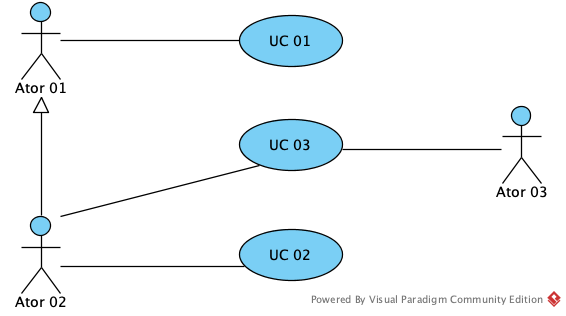
\includegraphics[width=.7\textwidth]{figuras/fig-casos-de-uso-subsistema-01.png}
	\caption{Diagrama de Casos de Uso do subsistema 01.}
	\label{fig-casos-de-uso-subsistema-01}
\end{figure}

A seguir, são apresentadas as descrições de cada um dos casos de uso identificados. Os casos de uso cadastrais de baixa complexidade, envolvendo inclusão, consulta, alteração e exclusão (CRUDs), são descritos na Tabela~\ref{tbl-casos-de-uso-subsistema-01-cruds}.

% Tabela de casos de uso cadastrais.
\begin{longtable}{|c|p{2.5cm}|p{6cm}|p{2.2cm}|p{2cm}|}
	\caption{Caso de uso cadastrais do subsistema 01.}
	\label{tbl-casos-de-uso-subsistema-01-cruds} \\\hline 
	
	% Cabeçalho e repetição do mesmo em cada nova página. Manter como está.
	\rowcolor{lightgray}
	\textbf{Id} & \textbf{Nome} & \textbf{Ações} & \textbf{Requisitos} & \textbf{Classes} \\\hline	
	\endfirsthead
	\hline
	\rowcolor{lightgray}
	\textbf{Id} & \textbf{Nome} & \textbf{Ações} & \textbf{Requisitos} & \textbf{Classes} \\\hline	
	\endhead
	
	% Especificar os atores abaixo, substituindo os exemplos.
	\UC\label{uc-subsistema-01-exemplo-01} & Caso de uso 01 & 
		\begin{itemize}[nosep,leftmargin=8mm]\vspace{-6mm}
			\item[(I)] Restrições de Inclusão;
			\item[(C)] Consulta;
			\item[(A)] Alteração;
			\item[(E)] e Exclusão.
		\vspace{-4mm}\end{itemize}
		& Listar os requisitos satisfeitos por este UC. 
		& Listar possíveis classes envolvidas.
		\\\hline

	\UC\label{uc-subsistema-01-exemplo-02} & Caso de uso 02 & 
		\begin{itemize}[nosep,leftmargin=8mm]\vspace{-6mm}
			\item[(I)] Sem restrições;
			\item[(C)] Sem restrições;
			\item[(A)] Atributos X, Y, Z não podem ser alterados;
			\item[(E)] Não disponível.
		\vspace{-4mm}\end{itemize}
		& \ref{rf-exemplo-01}, \ref{rf-exemplo-02}
		& Classe 01, Classe 02.
		\\\hline
\end{longtable}

Os casos de uso de consulta mais abrangente que as consultas a um único objeto, mas ainda de baixa complexidade, tais como consultas que combinam informações de vários objetos envolvendo filtros, estão descritos na Tabela~\ref{tbl-casos-de-uso-subsistema-01-consultas}.

% Tabela de casos de uso de consulta.
\begin{longtable}{|c|p{2.5cm}|p{6cm}|p{2.2cm}|p{2cm}|}
	\caption{Caso de uso de consultas envolvendo múltiplos objetos do subsistema 01.}
	\label{tbl-casos-de-uso-subsistema-01-consultas} \\\hline 
	
	% Cabeçalho e repetição do mesmo em cada nova página. Manter como está.
	\rowcolor{lightgray}
	\textbf{Id} & \textbf{Nome} &  \textbf{Descrição} & \textbf{Requisitos} & \textbf{Classes} \\\hline	
	\endfirsthead
	\hline
	\rowcolor{lightgray}
	\textbf{Id} & \textbf{Nome} &  \textbf{Descrição} & \textbf{Requisitos} & \textbf{Classes} \\\hline	
	\endhead
	
	% Especificar os atores abaixo, substituindo os exemplos.
	\UC\label{uc-subsistema-01-exemplo-03} & Caso de uso 03 & Descrição da consulta a ser realizada. & Listar os requisitos satisfeitos por este UC. & Listar possíveis classes envolvidas. \\\hline
	
	\UC\label{uc-subsistema-01-exemplo-04} & Caso de uso 04 & Descrição da consulta a ser realizada. & \ref{rf-exemplo-03} & Classe 03, Classe 04. \\\hline
\end{longtable}

Os casos de uso deste subsistema que não se encaixam nas categorias acima são descritos nas páginas subsequentes.


% Descrição de um caso de uso. 
% Reproduzir quantas forem necessárias para descrever os casos de uso que não se encaixarem como CRUDs ou consultas.
\clearpage
\begin{center}\textbf{Descrição de Caso de Uso}\end{center}

\noindent\textbf{Projeto:} \imprimirtitulo \\
\textbf{Identificador:} \UC\label{uc-subsistema-01-exemplo-05} \\
\textbf{Nome:} Caso de uso 05 \\
\textbf{Descrição:} descrição sucinta do propósito deste caso de uso.\\

% Tabela de descrição de um caso de uso.
\begin{longtable}{|p{2.3cm}|p{2.5cm}|p{10cm}|}
	\caption{Fluxos de eventos normais para o caso de uso 05.}
	\label{tbl-casos-de-uso-subsistema-01-exemplo-05} \\\hline 
	
	% Cabeçalho e repetição do mesmo em cada nova página. Manter como está.
	\rowcolor{lightgray}
	Cenário & Precondição & Descrição \\\hline	
	\endfirsthead
	\hline
	\rowcolor{lightgray}
	Cenário & Precondição & Descrição \\\hline
	\endhead
	
	% Especificar os cenários abaixo, substituindo os exemplos.
	Cenário 01 & Precondição do cenário 01 & 
	\begin{enumerate}[nosep,leftmargin=8mm]\vspace{-6mm}
			\item O ator faz algo;
			\item O sistema responde de certa forma;
			\item O ator reage de um jeito;
			\item O sistema etc...
	\vspace{-4mm}\end{enumerate} \\\hline

	Cenário 02 & Precondição do cenário 02 & 
	\begin{enumerate}[nosep,leftmargin=8mm]\vspace{-6mm}
		\item O ator faz algo;
		\item O sistema responde de certa forma;
		\item O ator reage de um jeito;
		\item O sistema etc...
	\vspace{-4mm}\end{enumerate} \\\hline
\end{longtable}


\noindent\textbf{Fluxos variantes:}\vspace{-4mm}
\begin{itemize}
	\item No \textbf{cenário 01}, no caso de \textbf{isso ou aquilo acontecer}, o sistema deve ...
\end{itemize}

\noindent\textbf{Requisitos relacionados:} \ref{rf-exemplo-01}, \ref{rf-exemplo-03}

\noindent\textbf{Classes relacionadas:} \hl{listar possíveis classes relacionadas}.
\newpage


% Definir uma subseção para cada subsistema.	
\section{Subsistema 02}
\label{sec-casos-de-uso-subsistema-02}

Etc...
\vspace*{1.5cm}

\chapter{Modelo Estrutural}
\label{sec-modelo-estrutural}
\vspace{-1cm}

O modelo conceitual estrutural visa capturar e descrever as informações (classes, associações e atributos) que o sistema deve representar para prover as funcionalidades descritas nos casos de uso especificados na Seção~\ref{sec-casos-de-uso}. 

A seguir, são apresentados os diagramas de classes de cada um dos subsistemas identificados no contexto deste projeto. Na Seção~\ref{sec-dicionario} --- Dicionário de Projeto --- são apresentadas as descrições das classes, atributos e operações presentes nos diagramas apresentados nesta seção.

\vitor{Para cada subsistema, apresentar um diagrama de classes em uma figura separada, introduzindo a figura no texto como no exemplo da Figura~\ref{fig-modelo-estrutural-subsistema-01}, abaixo.}

A Figura~\ref{fig-modelo-estrutural-subsistema-01} apresenta o diagrama de classes do subsistema 01.

\begin{figure}
	\centering
	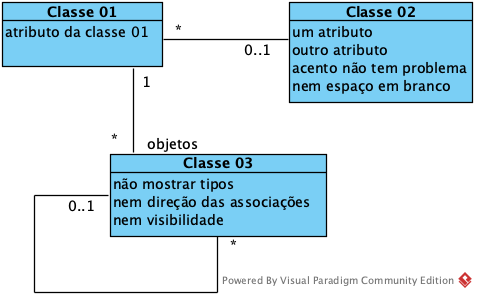
\includegraphics[width=.7\textwidth]{figuras/fig-modelo-estrutural-subsistema-01.png}
	\caption{Diagrama de classes do subsistema 01.}
	\label{fig-modelo-estrutural-subsistema-01}
\end{figure} 


% Replicar para outros subsistemas.
A Figura...


\vspace*{1.5cm}

\chapter{Dicionário de Projeto}
\label{sec-dicionario}

Esta seção apresenta as definições detalhadas das classes, descrevendo seus atributos e associações e servindo como um glossário do projeto. As definições são organizadas por subsistema, cada classe sendo apresentada em uma tabela separada. A coluna ``Obr.?'' indica com um ``x'' se o atributo é obrigatório (deve possuir um valor para se criar um objeto da classe).

Vale destacar que eventuais operações que estas classes vierem a ter não são listadas e descritas nesta fase do projeto. Além disso, na Seção~\ref{sec-modelo-estrutural}, algumas classes podem ser incluídas nos diagramas de outros subsistemas para ilustrar a relação entre eles. No dicionário de projeto, no entanto, classes são descritas apenas em seus subsistemas de origem.

\vitor{Criar uma subseção para cada subsistema. Dentro de cada subseção, criar uma tabela similar às tabelas~\ref{tbl-dicionario-subsistema-01-classe-01} e~\ref{tbl-dicionario-subsistema-01-classe-02}, abaixo, descrevendo as classes daquele subsistema. As linhas da tabela descrevem atributos e associações, explicando o que representam no domínio do problema. Os tipos devem ser genéricos (i.e., não específicos de uma linguagem de programação) e podem ilustrar também tipos específicos de domínio (ex.: CEP e CPF podem ser tipos de atributos). Quando a extremidade de uma associação possuir um nome, usar este nome na tabela (ex.: ``objetos'' na Tabela~\ref{tbl-dicionario-subsistema-01-classe-01}), do contrário usar um nome genérico dependendo da cardinalidade da extremidade. Não é necessário referenciar as tabelas em texto, pois a legenda de cada uma já indica qual classe está sendo descrita.}



% Definir uma subseção para cada subsistema.	
\section{Subsistema 01}
\label{sec-dicionario-subsistema-01}


% Tabela de dicionário de projeto referente a uma classe.
\begin{longtable}{|p{3.5cm}|c|c|p{8cm}|}
	\caption{Detalhamento da classe \emph{Classe 01}.}
	\label{tbl-dicionario-subsistema-01-classe-01} \\\hline 
	
	% Cabeçalho e repetição do mesmo em cada nova página. Manter como está.
	\rowcolor{lightgray}
	\textbf{Propriedade} & \textbf{Tipo} & \textbf{Obr.?} & \textbf{Descrição} \\\hline
	\endfirsthead
	\hline
	\rowcolor{lightgray}
	\textbf{Propriedade} & \textbf{Tipo} & \textbf{Obr.?} & \textbf{Descrição} \\\hline
	\endhead
	
	% Especificar os atributos e associações da classe abaixo, substituindo os exemplos.
	atributo da classe 01 	& Texto 	& x & Descrição do atributo da classe 01. \\\hline
	classe 02 				& Classe 02 &	& Descrição da associação com a Classe 02. \\\hline 
	objetos 				& Classe 03 &	& Associação com Classe 03 possui nome ``objetos''. \\\hline 
\end{longtable}


% Tabela de dicionário de projeto referente a uma classe.
\begin{longtable}{|p{3.5cm}|c|c|p{8cm}|}
	\caption{Detalhamento da classe \emph{Classe 02}.}
	\label{tbl-dicionario-subsistema-01-classe-02} \\\hline 
	
	% Cabeçalho e repetição do mesmo em cada nova página. Manter como está.
	\rowcolor{lightgray}
	\textbf{Propriedade} & \textbf{Tipo} & \textbf{Obr.?} & \textbf{Descrição} \\\hline
	\endfirsthead
	\hline
	\rowcolor{lightgray}
	\textbf{Propriedade} & \textbf{Tipo} & \textbf{Obr.?} & \textbf{Descrição} \\\hline
	\endhead
	
	% Especificar os atributos e associações da classe abaixo, substituindo os exemplos.
	um atributo				& Inteiro	& x & Descrição deste atributo. \\\hline
	outro atributo			& Real		& 	& Exemplos \\\hline
	acento não tem problema	& Data		& 	& de \\\hline
	nem espaço em branco	& Booleano	& x	& tipos de dados. \\\hline
	classes 01 				& Classe 01 &	& Descrição da associação com a Classe 01. \\\hline 
\end{longtable}



% Definir uma subseção para cada subsistema.	
\section{Subsistema 02}
\label{sec-dicionario-subsistema-02}

Etc...
\endgroup



% Finaliza a parte no bookmark do PDF para que se inicie o bookmark na raiz e adiciona espaço de parte no sumário.
\phantompart

% Marca o início dos elementos pós-textuais.
\postextual

\phantompart
\printindex

% Fim do documento.
\end{document}
